\documentclass[a4paper]{scrartcl}

%\usepackage{showframe}
\usepackage[margin=2cm,footskip=.7cm]{geometry}
\usepackage{enumitem}
% \usepackage{fourier}
\usepackage{xcolor}
% \usepackage{abkuerzungen}
\usepackage{hyperref}
\usepackage{amsmath}
\usepackage{ISASmacros/isasmathmacros}

\usepackage{pdfpages}


\newcommand{\sA}{\ensuremath{\mathsf{A}}}
\newcommand{\sAB}{\ensuremath{\mathsf{AB}}}
\newcommand{\sB}{\ensuremath{\mathsf{B}}}
\newcommand{\sBA}{\ensuremath{\mathsf{BA}}}
\newcommand{\sC}{\ensuremath{\mathsf{C}}}

\newcommand{\cest}{\ensuremath{\cvec{\gamma}}}
\newcommand{\cerest}{\ensuremath{\ervec{\gamma}}}
\newcommand{\cmat}{\ensuremath{\mat{\Gamma}}}
\newcommand{\tmat}{\ensuremath{\widetilde{\mat{\Gamma}}}}

\newcommand{\gainA}{\ensuremath{\mat{K}}}
\newcommand{\gainB}{\ensuremath{\mat{L}}}

% \newcommand{\fus}{\ensuremath{\op{fus}}}

% \newcommand{\CI}{\op{CI}\xspace}
% \newcommand{\EI}{\op{EI}\xspace}
% \newcommand{\ICI}{\op{ICI}\xspace}
% \newcommand{\BC}{\op{B\!/\!C}\xspace}
% \newcommand{\ind}{\op{s}\xspace}
\newcommand{\ind}{\op{in}\xspace}
\newcommand{\opt}{\cmat}


\newcommand{\excmat}{\ensuremath{\mat{\Gamma}'}}
\newcommand{\excest}{\ensuremath{\cest'}}
% \newcommand{\exoptmat}{\ensuremath{\mat{C}_{\excmat}}}
\newcommand{\exoptmat}{\ensuremath{\mat{C}'_\EI}}

%\RequirePackage[mathscr]{euscript}
%\RequirePackage{bbding}
%\RequirePackage{scalefnt}
%\RequirePackage{mathtools}
% This was enabled but makes the text look ugly
%\RequirePackage[T1]{fontenc}


%%% COLOR DEFINITIONS

% KIT Colors
\definecolor{kitgreenex}{RGB}{0,152,131}
\definecolor{kitblueex}{RGB}{52,115,186}
\definecolor{kitmaygreen}{RGB}{119,184,38}
\definecolor{kityellow}{RGB}{255,228,0}
\definecolor{kitorange}{RGB}{247,154,0}
\definecolor{kitbrown}{RGB}{182,130,28}
\definecolor{kitred}{RGB}{187,25,23}
\definecolor{kitpurple}{RGB}{190,0,126}
\definecolor{kitcyanblue}{RGB}{0,167,227}
% Own Definitions
\definecolor{grey}{RGB}{150,150,150}


\definecolor{nblue}{RGB}{54,95,145}

%%% FONTS
%\setkomafont{pageheadfoot}{\small\color{darkgray}}
%\setkomafont{pagefoot}{\normalfont\color{darkgray}}
%\setkomafont{pagenumber}{\color{darkgray}}
%\setkomafont{captionlabel}{\small\bfseries\color{darkgray}}
\setkomafont{disposition}{\bfseries}
\setkomafont{section}{\normalfont\large\bfseries}
\setkomafont{subsection}{\normalfont\bfseries}
\setkomafont{author}{\normalfont}
\setkomafont{date}{\normalfont}


%%% PARAGRAPH LAYOUT
\setlength{\parindent}{0mm}
\setlength{\parskip}{6pt}


%%% REBUTTAL COMMANDS
\newenvironment{rebuttal}{\begin{enumerate}[label={\color{grey}\thesection.\arabic{enumi}},leftmargin=0pt,ref=\thesection.\arabic{enumi}]}{\end{enumerate}}
\newcommand{\reviewtext}[1]{{\color{nblue} #1}}
\newcommand{\papertext}[1]{\emph{``#1''}}

%%% HYPERREF SETUP
\hypersetup{
        colorlinks = true,
        linkcolor = kitgreenex
}

%%%%%%%%%%%%%%%%%%%%%%%%%%%%%%%%%%%%%%%%%%%%%%%%%%%%%%%%%%%%%%%%%%%%%%%%

\title{\boldmath Cryptographically Privileged State Estimation With Gaussian Keystreams}
\subtitle{Response to Reviewers' Comments - Submission L-CSS 21-0154}
\author{Marko Ristic\and Benjamin Noack\and Uwe D. Hanebeck}

%       .d8888b.  888                     888
%      d88P  Y88b 888                     888
%      Y88b.      888                     888
%       "Y888b.   888888  8888b.  888d888 888888
%          "Y88b. 888        "88b 888P"   888
%            "888 888    .d888888 888     888
%      Y88b  d88P Y88b.  888  888 888     Y88b.
%       "Y8888P"   "Y888 "Y888888 888      "Y888



\begin{document}

\maketitle

Dear Dr. Ji-Feng Zhang,\\
Dear Reviewers,

We would like to thank you all for your thorough and helpful reviews. In this letter, we explain how the reviewer comments, questions, and suggestions have been addressed. Throughout this response, reviewers' comments are in \reviewtext{blue}. 

Sincerely,\\
Marko Ristic, Benjamin Noack, and Uwe D. Hanebeck

%      8888888888     888 d8b 888
%      888            888 Y8P 888
%      888            888     888
%      8888888    .d88888 888 888888 .d88b.  888d888
%      888       d88" 888 888 888   d88""88b 888P"
%      888       888  888 888 888   888  888 888
%      888       Y88b 888 888 Y88b. Y88..88P 888
%      8888888888 "Y88888 888  "Y888 "Y88P"  888



\section*{Response to the Editor's Report}
\def\thesection{E}
\begin{rebuttal} %\setcounter{enumi}{-1}
\item \reviewtext{The authors should address all the concerns, in particular:

- the proposed method seems not effective in the case there is some delay in the communication}

This is correct, the requirement for additional index information was neglected in the manuscript and has now been clarified. Our method relies on a cryptographic stream cipher which requires index information when communicating on a lossy channel. We have considered the case when all measurements arrive in order but have clarified the implications when communication delays or losses are present.

\item \reviewtext{- sometime it is hard to follow the  notations/definitions (in particular section II )}

We are sorry that the definitions and notations were not made easier to follow. Several equations, definitions, and the notation section have now been updated to make them clearer and to make Section II easier to understand. Additionally, we have clarified some of our reasoning in the reviewer responses below.

\item \reviewtext{As far as the paper acceptance at CDC, the reviewers are positive.}

We are glad to hear this, thank you.

\end{rebuttal}

%      8888888b.                         d888
%      888   Y88b                       d8888
%      888    888                         888
%      888   d88P .d88b.  888  888        888
%      8888888P" d8P  Y8b 888  888        888
%      888 T88b  88888888 Y88  88P        888
%      888  T88b Y8b.      Y8bd8P         888
%      888   T88b "Y8888    Y88P        8888888



\section*{Response to the Comments of Reviewer 1 (42339)}
\def\thesection{R1}
\begin{rebuttal}
\item \reviewtext{The authors present a framework in which different estimators can estimate the state with different confidence levels. They use pseudorandom Gaussian noise to corrupt the data stream for "unprivileged" estimators. However, legitimate estimators have access to the key used for generating the random number and can cancel its effect. 

The topic is interesting. The idea is simple and effective.}

We appreciate the supportive comment, thank you.

\item \reviewtext{My main criticism is the fragility of the proposed method. The slightest timing issues can cause massive errors down the line. If there is one time slot delay, the quality of the estimate at a legitimate estimator becomes twice as bad as the unprivileged estimator (since the measurement error at the legitimate estimator becomes z\_\{k\}-z\_\{k-1\}, which will be a zero mean Gaussian variable with covariance 2Z). This really restrict the use of the proposed method. Assuming that the encrypted/secure controller/estimator are of value in networked system, as also discussed in the introduction of the paper, the extreme sensitivity of the proposed method to even smallest delays (which are of course common occurrences in networked system) render the solution impractical.}

The criticism is justified. As an encryption method relying on an underlying stream cipher, index information is crucial for the correct decryption of sent data, and in our case, the correct removal of added noise. While some networked systems relying on an additional transfer protocol such as TCP/IP provide index (and thus time step $k$) information in sent packets, we have considered the simplified case where all sent measurements arrive, in order, and have neglected any additional index information. We failed to mention this in the work and thank you for pointing it out; some sentences have now been added in Section III.B which now clarifies the need for index information to be sent alongside measurements and states the context which we consider.

\item \reviewtext{I strongly encourage the authors to look into studies using pseudorandom noise generated by chaotic systems (e.g., 10.1007/978-981-15-0493-8\_6). The legitimate estimator uses a chaotic system that can be synchronized with the one at the transmitter to remove the effect of the noise. This idea is very similar to the proposed approach in the paper.}

Thank you for the suggestion, the paper indeed considers a very similar problem to our work. The key differences between this method and our own is the cryptographic guarantees presented in our work and the possible extension to multiple levels of privileged estimation. We have now added a reference and compared the method to our own in the introduction.

\end{rebuttal}

%      8888888b.                         .d8888b.
%      888   Y88b                       d88P  Y88b
%      888    888                              888
%      888   d88P .d88b.  888  888           .d88P
%      8888888P" d8P  Y8b 888  888       .od888P"
%      888 T88b  88888888 Y88  88P      d88P"
%      888  T88b Y8b.      Y8bd8P       888"
%      888   T88b "Y8888    Y88P        888888888



\section*{Response to the Comments of Reviewer 2 (42343)}
\def\thesection{R2}
\begin{rebuttal}
\item \reviewtext{This paper considers a method for allowing different users to have different state estimation qualities via the addition of pseudorandom Gaussian noise. The idea is that if one user has access to a secret key (a privileged user), then that user can construct and hence subtract the pseudorandrom noise from the received measurements. While if the user does not know the secret key (unprivileged user), the additional noise will degrade its estimation quality. The idea itself is quite simple though interesting. An extension to multiple privileges which involves multiple secret keys, is also given. 

Below are comments on the paper

The proposed scheme for the unprivileged user appears to have the same stability properties as the privileged user, so that if the privileged user has bounded error covariance then the unprivileged user also has bounded error covariance. Is it possible to have situations where the privileged user has bounded error covariance and the unprivileged user has unbounded error covariance?}

Thank you for the interesting comment. The idea of affecting the system stability by changing only the perceived measurement noise at an unprivileged estimator was initially explored but found not to work. The stability of a dynamical system is dependent on the reachability of $(\mat{F}, \mat{Q}^{\frac{1}{2}})$ and the observability of $(\mat{F}, \mat{H})$. The proof for this can be found in Chapter 11 of ``Random Processes in Systems - Lecture Notes'' by J. Walrand and A. Dimakis. For this reason, by artificially increasing the measurement noise $\mat{R}$ at an estimator ($\mat{R}+\mat{Z}$ substitutes $\mat{R}$ for the unprivileged estimator in our scheme) only the convergence value and the rate of convergence or divergence can be changed, rather than convergence itself.

\item \reviewtext{Another related work on adding noise to enhance security is ``On the Use of Artificial Noise for Secure State Estimation in the Presence of Eavesdroppers'', ECC 2018.}

Thank you for the suggestion. We had not found this paper during our literature review but see that it targets a very similar problem to the one we consider. We believe the key differences to our method are the cryptographic guarantees that we provide and the proposed extension to multiple levels of estimation privilege. We have now added a reference to the work in our introduction.

\item \reviewtext{p.2: In the definition of \$noise(sk, k, M\_S, M\_M,\textbackslash underline\{y\}\_1,\textbackslash dots, \textbackslash underline\{y\}\_k)\$, underlines are missing in ``measures \$y\_1,\textbackslash dots,y\_k\$}

Thank you for pointing this out, the mistake has now been fixed.

\item \reviewtext{In Definition 2.2, define what is meant by a ``negligible function''}

We apologize that this was left undefined. Due to the term's prevalence in cryptography and the manuscript space restraints, we have not repeated the definition in our work, but have now added a reference to its definition within Definition 2.2.

\item \reviewtext{p.4: In the Proof Sketch, write down a formal statement of the actual theorem that is to be proved}

Thank you for the suggestion. The section has now been updated to include the theorem being proved before the proof sketch.

\item \reviewtext{In Fig. 3, what exactly does  Priv.1, Priv.2 and Priv.3 mean? Does it
mean that it does not know one of the keys, while the other keys are
known?}

We are sorry that this was not made clear. The intention was that each privileged estimator holds a single secret key. We have changed the figure and its description to make this clearer.

\end{rebuttal}

%      8888888b.                         .d8888b.
%      888   Y88b                       d88P  Y88b
%      888    888                            .d88P
%      888   d88P .d88b.  888  888          8888"
%      8888888P" d8P  Y8b 888  888           "Y8b.
%      888 T88b  88888888 Y88  88P      888    888
%      888  T88b Y8b.      Y8bd8P       Y88b  d88P
%      888   T88b "Y8888    Y88P         "Y8888P"



\section*{Response to the Comments of Reviewer 3 (44309)}
\def\thesection{R3}
\begin{rebuttal}
\item \reviewtext{This paper introduces a method to decrease estimation quality at an unprivileged estimator using a stream of pseudorandom Gaussian samples while leaving privileged estimation unaffected and requiring no additional transmission beyond an initial key exchange.

The reviewer has the following specific comments.

1. In Section II.A, would the secret key sk be unique for given setup input models and security parameter?}

We regret that this was not made clearer. There is no requirement for a privileged estimation scheme to produce a unique secret key given fixed inputs, and we have now clarified this by pointing out that the Setup and Noise algorithms may be probabilistic. The instance of a privileged estimation scheme that we propose in Section 3 is an example of this case, as the key is chosen at random given the security parameter and is not fixed. Similarly, Definition 2.3 takes probabilities over the randomness introduced in the Setup and Noise algorithms for this reason.

\item \reviewtext{2. The authors should better reorganise the problem statement part and make the definitions and notations more clearly. For example, the function A(.,.,.) is not defined before usage.}

We are sorry that the problem statement was not made clear. Due to the novelty of the cryptographic requirements, we believe there is a need for a suitable cryptographic problem to be formally defined alongside the estimation problem to which we propose a solution. As is common in cryptography, security notions are defined as broadly as possible, minimizing the assumptions on attackers and restrictions on implementations. For this reason, the problem statement has been given in its two distinct subsections, detailing a novel and reusable cryptographic security notion first, before a specific estimation problem where it can be used. We have made several minor changes to portray this intention further, including an added reference, corrected equations, and an updated notation section. We hope this has made the structure clearer.

\item \reviewtext{3. Could the setup cover other Gaussian keystream instead of the one the authors proposed in Section III.A?}

The idea behind our proposed privileged estimation scheme would work with any Gaussian keystream, however, to meet the security notion defined it is required that the Gaussian keystream is indistinguishable from random independent Gaussian samples to a polynomially bound attacker. For this reason, the method described has been used (given our assumptions about floating-point numbers, it meets the requirement) and is relied on in our later proof. An alternative Gaussian keystream providing the same guarantee could always replace the one we give, but the reliance on the well studied and replaceble component of a stream cipher reduces the security to a tried-and-tested method. We have added some minor changes that imply that the choice of our keystream is intentional but not compulsory.

\end{rebuttal}

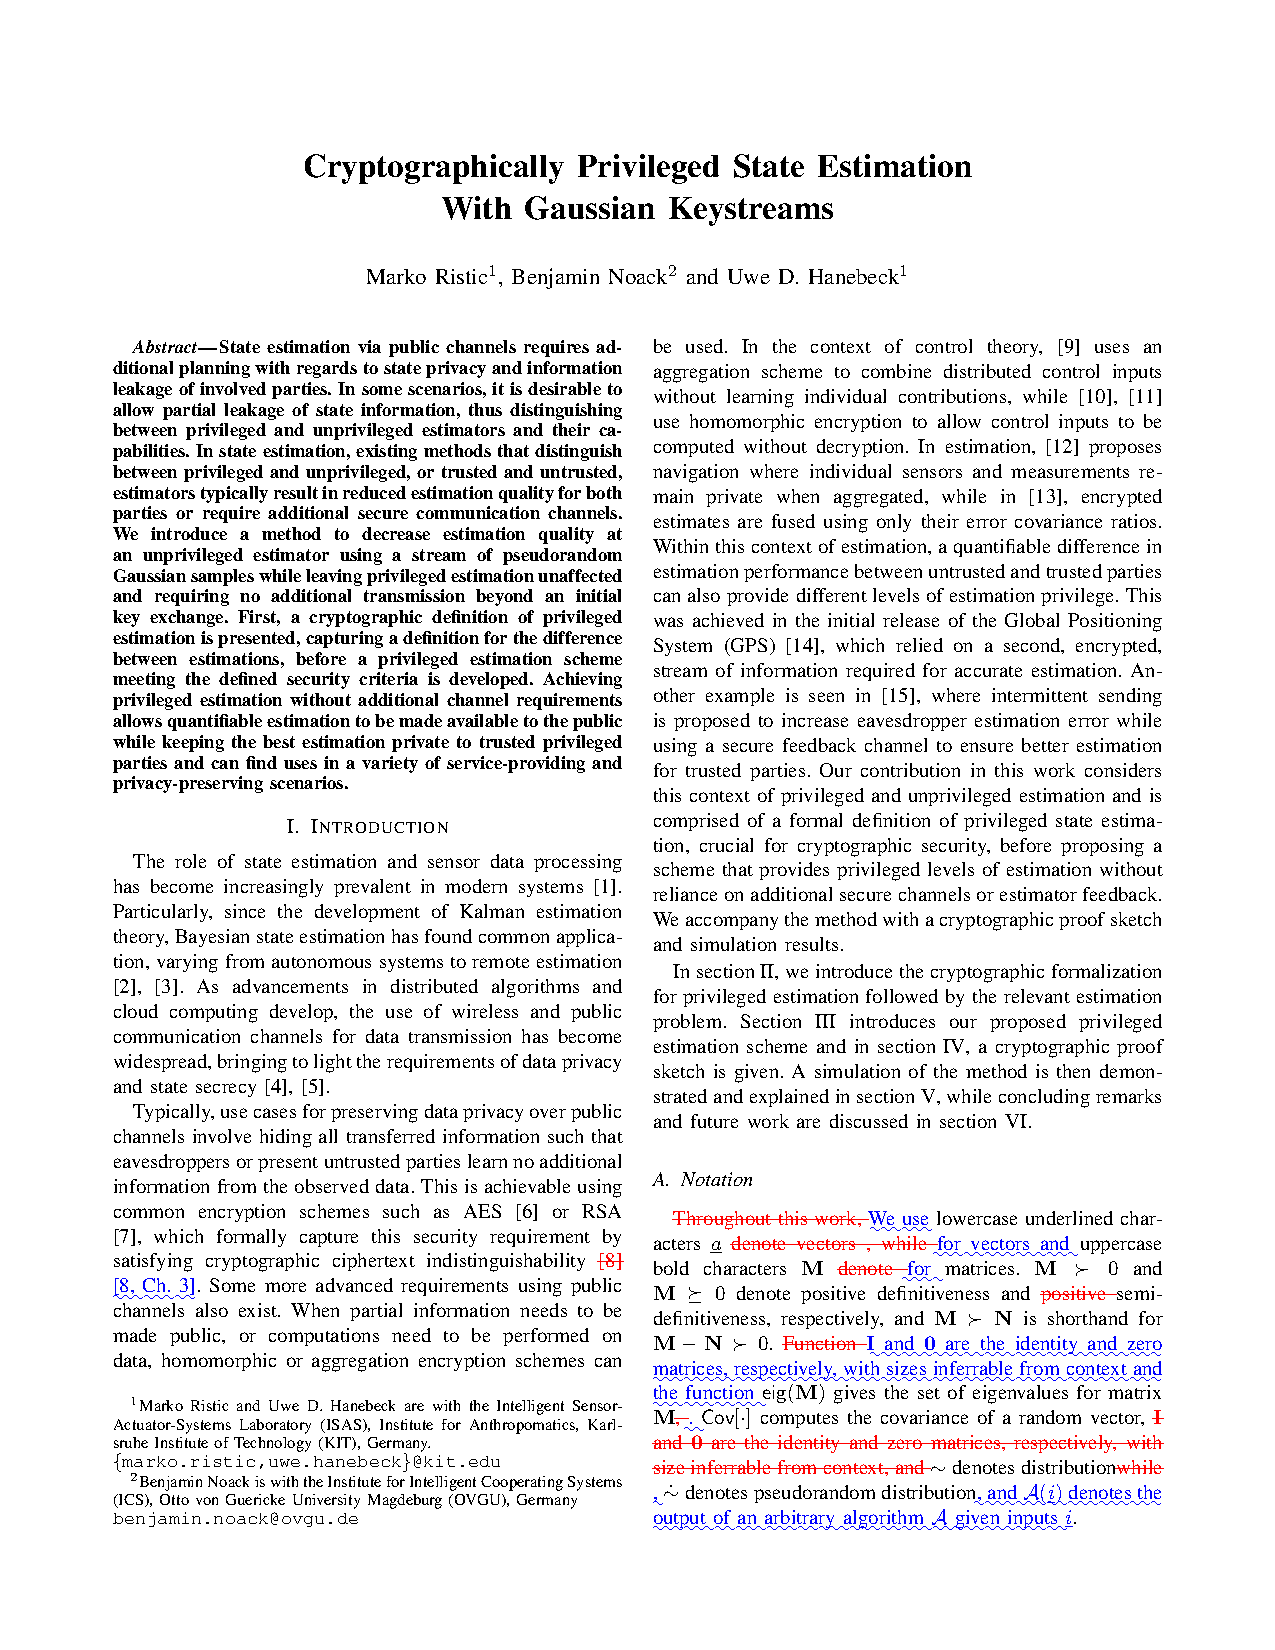
\includepdf[pages=-]{diff}

\end{document}